\documentclass{ledger}

%AUTHOR: This is a bare-bones template into which you may put your paper to aid in formatting your submission to Ledger. Note that to work properly, you must have the files "ledger.cls", "ledgerbib.bst", and the folder "images" on hand. 

%AUTHOR: the preferred method to generate PDF output is to use 'pdflatex'
%To clean up after a successful build, try: 'latexmk -c main.tex'

%EDITOR: in ledger.cls replace logoNewUC.png with logoNew.png prior to publication 


%EDITOR: replace X's to set the data for the header and footer
\newcommand{\thefirstpagenum}[0]{X}
\newcommand{\thelastpagenum}[0]{X}
\newcommand{\theyear}[0]{20XX}
\newcommand{\thevol}[0]{X}
\newcommand{\thedoi}[0]{DOI 10.5195/LEDGER.\theyear.XXX}
\newcommand{\ledgerpages}[0]{\thefirstpagenum-\thelastpagenum}


%AUTHOR: please set these to generate correct PDF metadata
\hypersetup{pdfauthor={Sun, Ephraim T.; 
Gijsbertsen, Laurens C.}, pdftitle={A Study on State-of-the-Art Alternative Asset Models and Their Application to Digital Assets}}

%EDITOR: set the correct pageination during layout
%\setcounter{page}{\thefirstpagenum}


%AUTHOR: this can be used to highlight changed text, surround with \edit{} and
%uncomment either to determine color
%\newcommand{\edit}[1]{{\color{red} #1}}
\newcommand{\edit}[1]{#1}
	
\overfullrule=10pt

\title{A Study on State-of-the-Art Alternative Asset Models and Their Application to Digital Assets
}
\author{Dr. Simon Mak\thanks{S. Mak (smak@smu.edu) - Faculty Advisor, Director of the Caruth Institute for Entrepreneurship}, Ephraim T. Sun\thanks{E. Sun (ephraims@smu.edu)} , Laurens C. Gijsbertsen,\thanks{L. Gijsbertsen (lgijsbertsen@smu.edu)}}

\pagestyle{pagemain}


%The Author should select the appropriate pretitle below:
\pretitle{
  \centering \selectfont LEDGER \LaTeX \ TEMPLATE \par
  %\centering \selectfont REVIEW ARTICLE \par
  %\centering \selectfont RESEARCH ARTICLE \par 
  %The Author should not remove the following text:
  Submission Under Consideration at Ledger \par 
  \fontsize{24pt}{28pt}\selectfont} % Title is centered and at 24pt


\begin{document}

\maketitle

\thispagestyle{pagefirst}

\begin{abstract}
This research project aims to conduct a comprehensive study on state-of-the-art alternative asset models and their application to digital assets. As the financial landscape continues to evolve, alternative assets, specifically digital assets, are gaining significant attention, and becoming increasingly relevant for investors. However, there is a lack of rigorous research and understanding of the various alternative asset investment models and their implications for digital assets. The primary research question driving this study is: "\textit{To what extent can existing alternative asset investing models be applied to digital assets?}" By examining and analyzing various alternative asset models, this research project seeks to assess the feasibility and effectiveness of applying these models to digital assets.

%AUTHOR: keywords are OK to show for Review article, will be hidden and added to metadata for publication
\begin{keywords}
\item State-of-the-art.
\item Alternative asset models.
\item Digital assets.
\item Cryptocurrency.
\item Application.
\item Feasibility.
\item Effectiveness.
\item Portfolio theory.
\item Factor-based models.
\item Risk management.
\end{keywords}
\end{abstract}

\section{Comprehensive Literature Review}
\subsection{Background}
Digital assets have grown rapidly in recent years, with the total market cap of cryptocurrencies surpassing \$2 trillion in 2021. While digital assets hold promising investment opportunities, the volatile and decentralized nature of this new asset class presents unique investment challenges compared to traditional assets. As investor interest in digital assets continues to grow, there is a need to explore best practices for evaluating and managing risks associated with digital asset investments.

Alternative asset investing offers strategies that may help address some of the challenges with digital assets. However, applying traditional alternative asset models directly to digital assets is not straightforward given key differences in their characteristics. It is therefore important to examine existing models and understand how they may need to be adapted for the digital asset landscape.

\subsubsection{Alternative Asset Models}
A wide range of alternative asset investing models have been developed and applied across various private market asset classes such as private equity, private credit, real assets and hedge funds. Common models used include portfolio theory, factor models, mean-variance optimization, and risk parity frameworks.

While these models have proven valuable in traditional alternative investments, it remains unclear whether and how they can be applied to digital assets. Digital assets such as cryptocurrencies differ significantly from traditional assets in factors like volatility, liquidity profile and regulatory oversight (FINRA.org).

\subsection {Digital Assets}
Cryptocurrencies were the first widely adopted digital assets, with Bitcoin being the largest. Since then, new digital asset classes have emerged including security tokens representing asset ownership, and utility tokens providing access to a network or platform.

Digital assets present both opportunities and challenges from an investment perspective. While some studies show they can provide portfolio diversification benefits, their short history makes volatility and risk difficult to assess over long periods (FINRA.org). Regulatory ambiguity also introduces legal and compliance complexities for investors (CRS Reports, 2023).

Connecting these concepts, there is a need for research exploring whether and how existing alternative asset investing approaches could benefit the growth of a regulated digital asset investment industry. This paper aims to address this gap by systematically analyzing various models and evaluating their applicability to different digital asset classes.

\section{Examining Existing Alternative Asset Models and Their Key Principles}

Blah blah blah. This paper is broken into the following sections.
\begin{itemize}
       \item[1] Risk and Return Analysis
            \begin{itemize}
            \item[1.1] Capital Asset Pricing Model (CAPM)
            \end{itemize}
       \item[2] Volatility Analysis
            \begin{itemize}
            \item[2.1] Generalized AutoRegressive Conditional Heteroskedasticity (GARCH)
            \item[2.2] Stochastic Model - Geometric Brownian Motion (GBM)
            \end{itemize}
       \item[3] Valuation Techniques
            \begin{itemize}
            \item[3.1] Relative Valuation Models - Network Value to Transactions (Comparative Analysis)
            \item[3.2] Absolute Valuation Models - Equation of Exchange (Intrinsic Value)
            \end{itemize}
       \item[4] Portfolio Management Strategies
            \begin{itemize}
            \item[4.1] Modern Portfolio Theory
            \end{itemize}
       \item[5] Price Prediction
           \begin{itemize}
           \item[5.1] Long Short Term Memory (LSTM)
           \item[5.2] Autoregressive Integrated Moving Average (ARIMA)
           \end{itemize}
\end{itemize}
% \begin{figure}
% \centering
% \captionsetup{justification=centering}
% 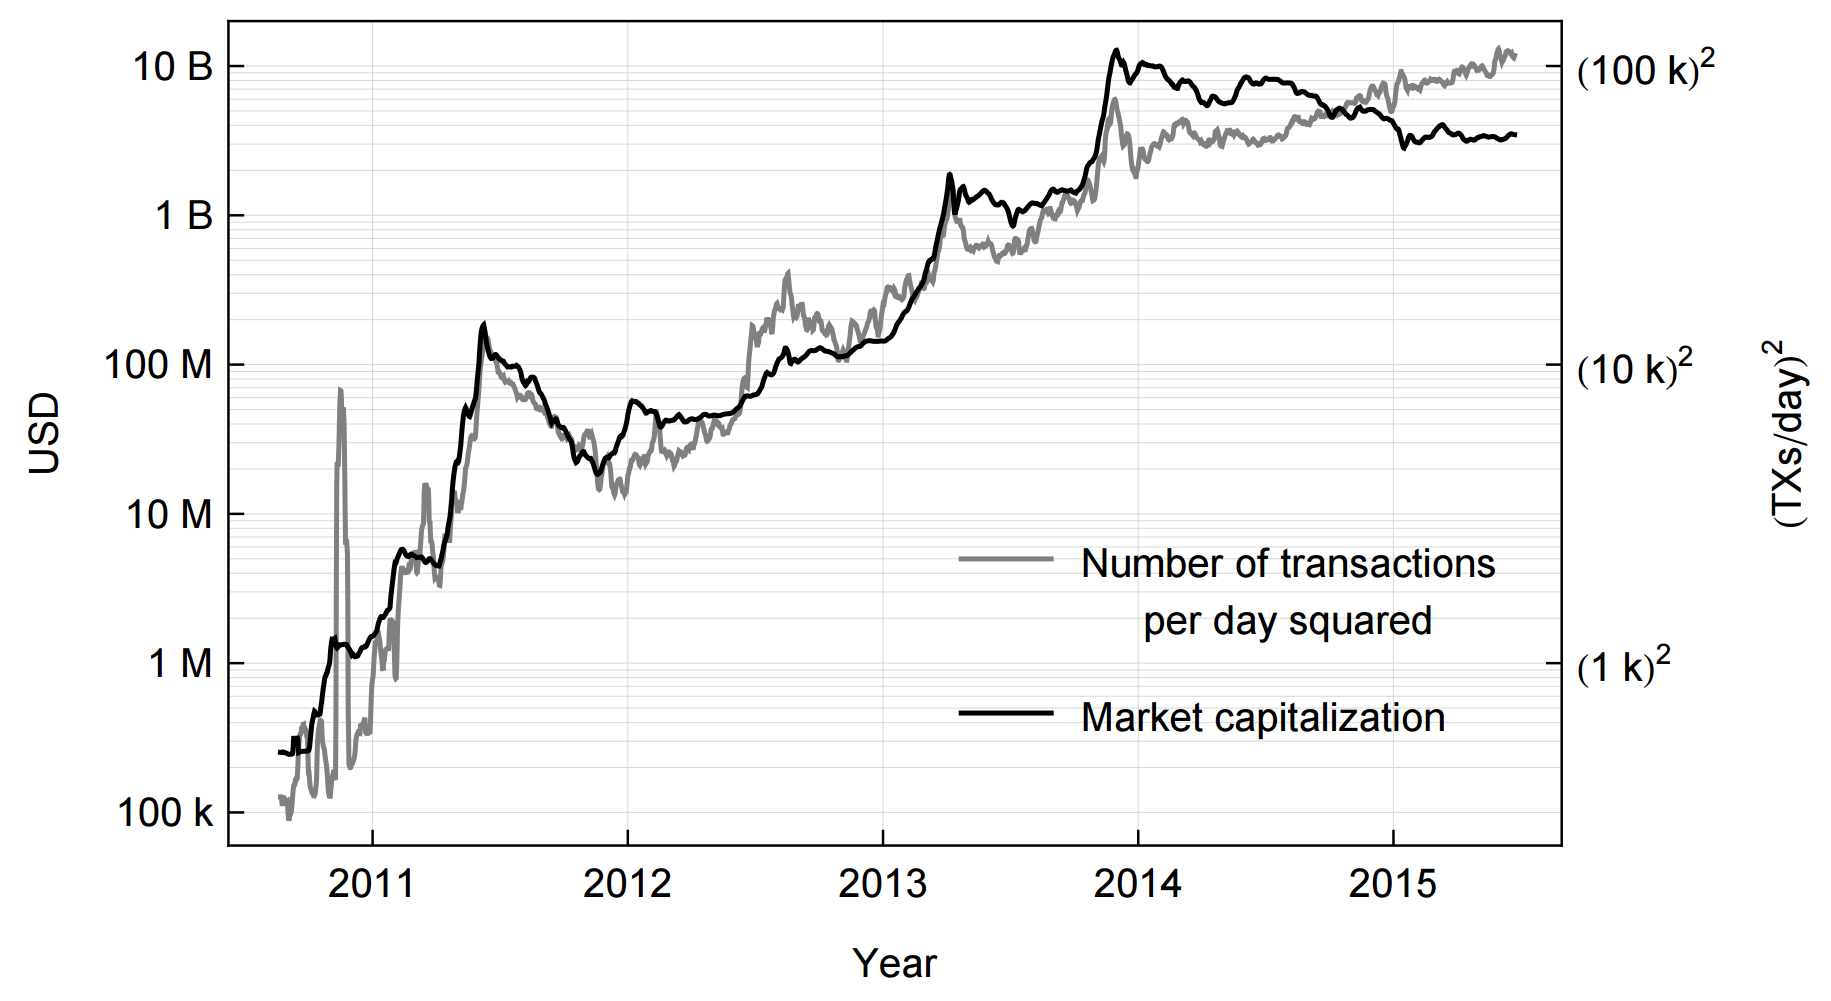
\includegraphics[width=1\textwidth]{graph.png}
%     \caption{A graph showing things of interest.}
%     \label{graph1}
% \end{figure}


\section{Digital Asset Landscape, Exploring the Unique Characteristics and Challenges associated with Investing in Digital Assets}

Info needed here.

\section{Data Preparation}

We decided to retrieve the top 10 best cryptocurrencies based on market cap as of 05/11/2024. We have excluded stablecoins like Tether (USDT) and USDC. Therefore, we have the following coins in order of market capitalization (excluding stablecoins): 
1) Bitcoin (BTC)
2) Ethereum (ETH)
3) Solana (SOL)
4) Binance Coin (BNB)
5) XRP (XRP)
6) Toncoin (TON)
7) Dogecoin (DOGE)
8) Cardano (ADA)
9) Shiba Inu (SHIB)
10) Avalanche (AVAX)

From the above list, we notice that we have the two main cryptocurrencies Bitcoin and Ethereum, with Bitcoin around \$1.2 trillion in value (according to CoinMarketCap) and Ethereum hovering around \$3.5 billion, about 3x less the value compared to Bitcoin.

The data is fetched from Yahoo Finance via yfinance. \cite{yfinance}. In terms of dates, unless otherwise specified, the default dates from Jan 1st, 2022 to Jan 1st, 2024. We use the daily adjusted close data as our data points, which is ample to provide various analysis.

\section{Risk and Return Analysis}

Investing in alternative assets offers unique opportunities and challenges, particularly in the realm of risk and return. Unlike traditional assets such as stocks and bonds, alternative assets—including private equity, hedge funds, real estate, and commodities—often exhibit different risk profiles and return characteristics. This distinct behavior necessitates a thorough analysis to understand how these assets can fit into an overall investment strategy and contribute to portfolio diversification and performance.

When assessing the risk and return of alternative assets, it is crucial to consider factors such as liquidity risk, market risk, and operational risk, which may differ significantly from those associated with traditional investments. Additionally, the return potential of alternative assets can be influenced by factors such as leverage, market inefficiencies, and unique economic exposures.

To systematically evaluate the risk and return characteristics of alternative assets, financial models and theories can be employed. One of the foundational models in finance for assessing the relationship between risk and expected return is the Capital Asset Pricing Model (CAPM).

The Capital Asset Pricing Model (CAPM) is a cornerstone of modern financial theory, providing a framework for understanding the trade-off between risk and return for individual assets in a diversified portfolio. Developed by William Sharpe in the 1960s, CAPM posits that the expected return of an asset is directly related to its systematic risk, as measured by beta (\(\beta\)). Beta represents the sensitivity of an asset's returns to the returns of the overall market, capturing the asset's exposure to market-wide risk factors.

According to CAPM, the expected return on an asset can be expressed as:

\[
E(R_i) = R_f + \beta_i (E(R_m) - R_f)
\]

where:

$ \bullet E(R_i) $ is the expected return of the asset,

$ \bullet R_f $ is the risk-free rate,

$ \bullet \beta_i $ is the beta of the asset,

$ \bullet E(R_m) $ is the expected return of the market,

$ \bullet E(R_m) - R_f $ is the market risk premium.


\hfill \break

\paragraph{Calculating CAPM for Cryptocurrencies}

\hfill \break

1. Determine the Risk-Free Rate (\(R_f\))

The risk-free rate is typically the return on government bonds, such as U.S. Treasury bills. For cryptocurrencies, we used the yield on a 10-year U.S. Treasury bond as a proxy for the risk-free rate.

2. Calculate the Expected Market Return (\(R_m\))

The expected market return can be the average return of a broad cryptocurrency market index. For this instance, we used the Bitwise 10 Crypto Index Fund (BITW) \cite{bitw}.

3. Calculate the Beta (\(\beta\))

Beta measures the volatility of a cryptocurrency relative to the market. 

To calculate beta:

\begin{itemize}
    \item Collect Historical Price Data: Obtain historical daily prices for each cryptocurrency and the chosen market index.
    \item Calculate Returns: Compute the daily returns for each cryptocurrency and the market index.
    \item Run a Regression Analysis: Perform a linear regression with the cryptocurrency returns as the dependent variable and the market index returns as the independent variable. The slope of the regression line is the beta.
\end{itemize}

4. Compute the Market Risk Premium (\(R_m - R_f\))

The market risk premium is the difference between the expected market return and the risk-free rate.

\paragraph{Analysis of Cryptocurrencies}

\begin{table}[h]
    \centering
    \begin{tabular}{ccc}
         \textbf{Asset} & \textbf{Beta} & \textbf{Market Risk Premium} \\
         \hline
         BTC-USD & 0.468009 & 0.062761 \\
         ETH-USD & 0.544777 & 0.068134 \\
         SOL-USD & 0.725297 & 0.080771 \\
         BNB-USD & 0.394427 & 0.057610 \\
         XRP-USD & 0.569858 & 0.069890 \\
         TON-USD & 0.415367 & 0.059076 \\
         DOGE-USD & 0.499549 & 0.064968 \\
         ADA-USD & 0.554140 & 0.068790 \\
         SHIB-USD & 0.523131 & 0.066619 \\
         AVAX-USD & 0.606193 & 0.072434 \\
    \end{tabular}
    \caption{Caption for the table}
    \label{tab:my_label}
\end{table}

\begin{figure}
    \centering
    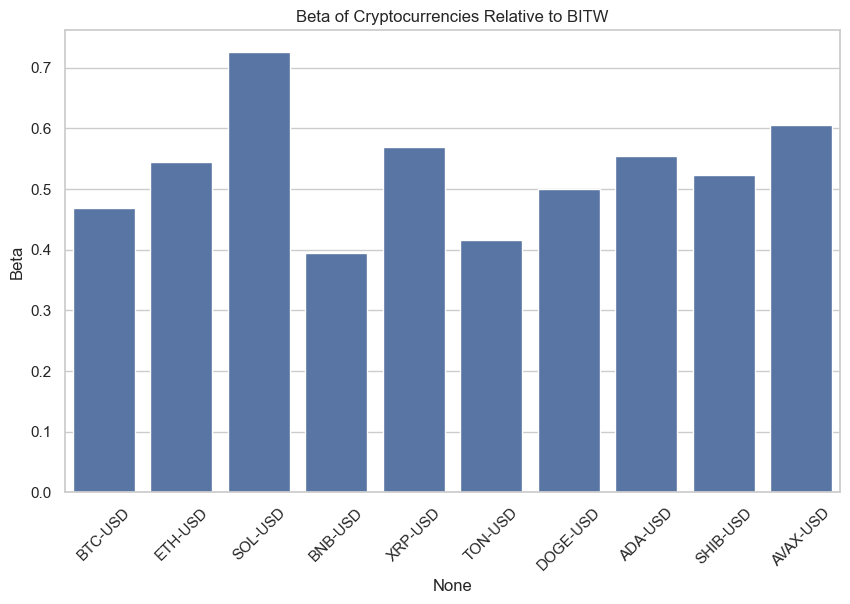
\includegraphics[width=0.8\textwidth]{./code/risk-and-return-analysis/capm/beta.png}
    \caption{Beta of Cryptocurrencies Relative to BITW}
    \label{fig:beta}
\end{figure}

\begin{figure}
    \centering
    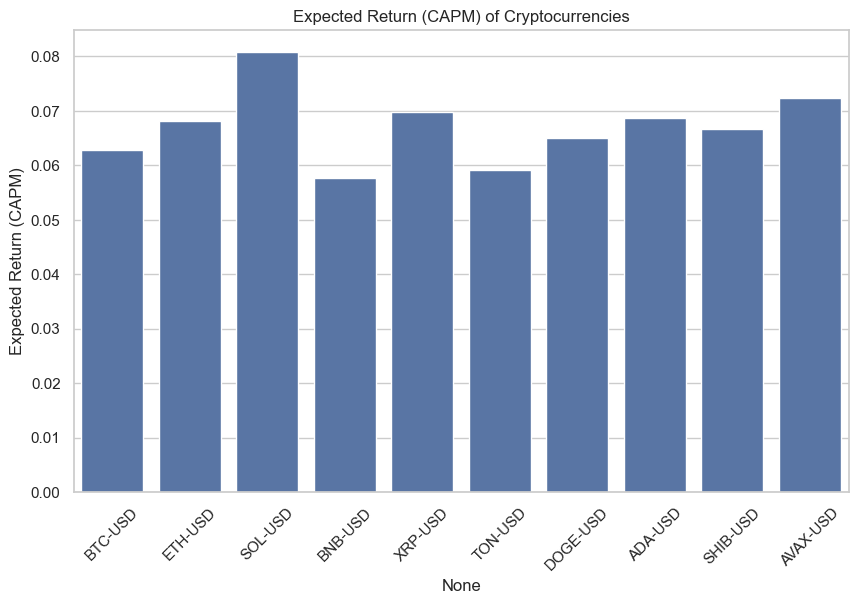
\includegraphics[width=0.8\textwidth]{./code/risk-and-return-analysis/capm/exp_return.png}
    \caption{Expected Return of Cryptocurrencies Relative to BITW}
    \label{fig:exp_return}
\end{figure}

\section{Volatility Analysis}

Volatility analysis plays a crucial role in understanding the behavior of financial assets, particularly in the realm of alternative investments. Volatility, often regarded as a measure of risk, encapsulates the degree of uncertainty or variability in the returns of an asset over time. In the context of alternative assets, which encompass a diverse range of investment vehicles beyond traditional stocks and bonds, volatility assumes heightened significance due to the unique characteristics and dynamics inherent in these assets.

The emergence of digital assets, such as cryptocurrencies and tokenized securities, has further underscored the importance of volatility analysis in alternative asset management. These nascent and rapidly evolving asset classes exhibit distinct patterns of price fluctuations and risk profiles, necessitating sophisticated analytical tools to model and assess their volatility dynamics accurately.

Volatility analysis serves multiple purposes in the management of alternative assets. Firstly, it provides insights into the inherent risk associated with these assets, enabling investors and portfolio managers to make informed decisions regarding asset allocation, risk mitigation strategies, and portfolio diversification. Secondly, volatility analysis facilitates the estimation of potential returns and the pricing of derivative instruments, such as options and futures, which are commonly utilized in alternative asset markets for hedging and speculation purposes.

Two prominent methodologies employed in volatility analysis are the Generalized Autoregressive Conditional Heteroskedasticity (GARCH) model and Stochastic Geometric Brownian Motion (GBM). The GARCH model, a time-series econometric framework, is widely utilized to model the volatility clustering and persistence observed in financial asset returns. By capturing the conditional heteroskedasticity of asset returns, the GARCH model enables practitioners to forecast future volatility levels accurately and assess the risk-return characteristics of alternative assets.

On the other hand, stochastic GBM, a stochastic process widely used in mathematical finance, provides a continuous-time framework for modeling the evolution of asset prices and their associated volatility. By incorporating random fluctuations and drift components into the asset price dynamics, stochastic GBM offers a versatile approach to simulating the behavior of alternative assets under various market conditions and investment scenarios.

\subsection{Stochastic Model - GBM}

\hfill \break

The Geometric Brownian Motion (GBM) is a model used in finance to describe the random movement of asset prices. It's represented by the equation:

\[
dS_t = \mu S_t dt + \sigma S_t dW_t
\]

Where:

$ \bullet S_t $ is the price of the asset at time $ t $.
 
$ \bullet \mu $ is the average rate of return, or drift.

$ \bullet \sigma $ is the volatility, or standard deviation of returns.

$ \bullet dW_t $ represents the random fluctuation in the asset's price.

\hfill \break

This equation states that the change in the asset price over a small time interval \( dt \) consists of two components: a deterministic component represented by \( \mu S_t dt \), and a random component represented by \( \sigma S_t dW_t \).



\begin{table}[h]
    \centering
    \begin{tabular}{ccc}
         \toprule
         \textbf{Asset} & \textbf{Mean} & \textbf{Standard Deviation} \\
         \midrule
         BTC-USD & 34831.378123 & 12556.081916 \\
         ETH-USD & 2186.967729 & 863.545155 \\
         SOL-USD & 55.782474 & 55.221616 \\
         BNB-USD & 323.091985 & 117.789668 \\
         XRP-USD & 0.631261 & 0.287855 \\
         TON-USD & 3.99546 & 3.533988 \\
         DOGE-USD & 0.125877 & 0.094779 \\
         ADA-USD & 0.829737 & 0.632222 \\
         SHIB-USD & 0.000013 & 0.000011 \\
         AVAX-USD & 32.960283 & 28.309159 \\
         \bottomrule
    \end{tabular}
    \caption{Summary Statistics of Selected Digital Assets}
    \label{tab:summary_stats}
\end{table}

\subsection{GARCH Model}

\hfill \break

The GARCH model is an econometric model that captures the time-varying volatility or variance of a time series. It assumes that the volatility of the series is autocorrelated and can be predicted based on past values of the series and past volatility.

The basic form of the GARCH(p, q) model is:

\[
\sigma_{t}^2 = \omega + \alpha_{1}\varepsilon_{t-1}^2 + \ldots + \alpha_{p}\varepsilon_{t-p}^2 + \beta_{1}\sigma_{t-1}^2 + \ldots + \beta_{q}\sigma_{t-q}^2
\]

Where:

$ \bullet \sigma_{t}^2 $ is the conditional variance at time $ t $,

$ \bullet \omega $ is the constant term,

$ \bullet \varepsilon_{t} $ is the error term at time $ t $,

$ \bullet \alpha_{i} $ and $ \beta_{i} $ are the coefficients for the squared error terms and the conditional variances at lag $ i $ respectively,

$ \bullet p $ and $ q $ are the orders of the autoregressive and moving average terms respectively.


\section{Valuation Techniques}

Need more info.

\section{Price Prediction}

Need more info.

\section{Portfolio Management Strategies}

Need more info.

\section{Analysis of Different Alternative Asset Models and Their Potential Application to Digital Assets}

Need More Info.

%define the following sections to hide their Section Number (Notes Style)
\ledgernotes

\section*{Acknowledgements} 

We would like to express our sincere gratitude to Dr. Simon Mak for his invaluable guidance and support in both the SMU Blockchain Club and this research paper. We also wish to acknowledge the SMU Blockchain Club community for their support and collaboration, which were instrumental to this work. Special thanks go to the Engaged Learning Fellowship Program, particularly Jennifer Ebinger, Senior Director, and Adam Neal, Program Manager, for their encouragement and assistance. Lastly, we extend our heartfelt thanks to Southern Methodist University for their generous financial support.

\section*{Author Contributions}

State the contribution made by each author.  Refer to authors using their initials, for example, ``FAL developed the code to perform the simulation (65\%) and FQL analyzed the results (35\%).  They both contributed equally to manuscript preparation.''

\section*{Conflict of Interest}

Authors should state any conflict of interest as defined by Ledger's Conflict of Interest Policy, available on the Ledger website. If the author believes there are no conflicts of interest, they should include the following: ``The author declares that they have no known conflicts of interest as per the journal’s Conflict of Interest Policy.''

%AUTHOR: comment out if using thebibliography
%\theendnotes

%AUTHOR: please read ledgerbib.bst usage notes by opening it in a text editor. We have modified it to include the use of the @misc item type for the proper formatting of online sources.

\bibliographystyle{ledgerbib}
\bibliography{tempbib}

%AUTHOR: comment out, this is used to make sure the Creative Commons License
%image fits on page

\newpage 	
%define the following sections to have the Appendix Style

\appendix
\setcounter{section}{0}
\section{Data and Descriptions}

\vspace{12pt}
\begin{table}[h]
\begin{center} 
\scalebox{0.6}{ 
\begin{tabular}{p{5cm}p{18cm}}%{l|}%{|>m{5cm}|>m{15cm}|}
%\rowcolor{orange}
\hline
 \textbf{Column A}  & \textbf{Column B} \\\hline
	Data & Description of data in more detail.\\
\hline
 Also Data & More description of data.\\
\hline 
 A Third Item & Pretium fusce id velit ut tortor pretium viverra suspendisse potenti. Enim sed faucibus turpis in eu. In hac habitasse platea dictumst quisque sagittis. Pharetra et ultrices neque ornare aenean euismod elementum.\\
\hline
%\hline
\end{tabular}}



\caption{A table in an appendix} \label{AppendixTable}
\end{center}
\end{table} 
%\newpage
%here up^^


\thispagestyle{pagelast}





%\theendnotes

\end{document}
